\documentclass[12pt, a4paper]{article}

% --- PACKAGES ---
\usepackage[utf8]{inputenc}
\usepackage[T1]{fontenc}
\usepackage[a4paper, margin=2.5cm]{geometry}
\usepackage{amsmath, amssymb, graphicx, float}
\usepackage{authblk}
\usepackage[square, numbers]{natbib}
\usepackage{hyperref}
\usepackage{caption}

% --- DOCUMENT INFORMATION ---
\title{A Cosmological Model without Dark Energy via an Evolving Time Rate Induced by Structure Formation}

\author[1]{Milen Krumov\thanks{Corresponding author: \href{mailto:krumov.milen@gmail.com}{krumov.milen@gmail.com}}}
\affil[1]{Independent Researcher, Bulgaria (ORCID: \href{https://orcid.org/0009-0008-3F57-9060}{0009-0008-3957-9060})}

\date{\today}

% --- HYPERLINK SETUP ---
\hypersetup{
    colorlinks=true, linkcolor=blue, urlcolor=cyan, citecolor=green,
    pdftitle={A Cosmological Model without Dark Energy},
}

% --- DOCUMENT START ---
\begin{document}
\maketitle

\begin{abstract}
We present a novel cosmological framework, the Phase-transition Linear Model (PLM-FP), that explains the observed cosmic acceleration without requiring dark energy. The model's core postulate is that the physical rate of time evolves dynamically as a function of the ambient energy density, a process driven by large-scale structure formation. We test this model against a comprehensive set of observational data: the Pantheon+ supernova catalog \cite{PantheonPlus}, Baryon Acoustic Oscillation (BAO) measurements \cite{BAO_compilation}, and Cosmic Microwave Background (CMB) distance priors from Planck 2018 \cite{Planck2018}. An MCMC analysis reveals that the PLM-FP model provides a statistically superior fit to the data compared to the standard $\Lambda$CDM model, with a $\Delta$BIC of approximately -5.46 million. The model naturally predicts a local blueshift effect of $z_{\text{local}} \approx -0.05$ and makes a falsifiable prediction for the global Hubble constant, $H_0 \approx 47.3$ km/s/Mpc. Our results demonstrate that a physically motivated model of dynamic time offers a compelling, self-consistent, and statistically preferred alternative to the dark energy paradigm.
\end{abstract}

\section{Introduction}
The standard cosmological model, $\Lambda$CDM, has been remarkably successful in describing a wide range of astronomical observations. However, its foundation rests upon two hypothetical entities---dark matter and dark energy---which constitute 95\% of the Universe's energy budget but whose fundamental nature remains unknown. Furthermore, the growing ``Hubble tension'' \cite{Riess2021} suggests that the $\Lambda$CDM model may be incomplete. In this work, we explore an alternative based on the postulate that the rate of physical time is not a universal constant but a dynamic quantity linked to the local energy density of the medium through which information propagates. We propose that structure formation drives an evolution in the rate of time, which in turn affects our measurements of cosmological distances, creating the illusion of accelerated expansion.

\section{The PLM-FP Model Formulation}
The model is built upon the FLRW metric but introduces new dynamics by modifying the expansion history, $H(z)$.

\subsection{Partition of Energy Components}
We partition the total matter density $\Omega_m$ into a ``bound'' component and a ``free'' component. The fraction of bound matter, $f_{\text{bound}}(z)$, is modeled as:
\begin{equation}
f_{\text{bound}}(z) = f_{\max} \cdot \frac{1}{2} \left[1 - \tanh\left(\frac{z - z_{\text{crit}}}{w_{\text{crit}}}\right)\right]
\end{equation}
The energy density of the free component, $\Omega_{\text{free}}(z)$, is then:
\begin{equation}
\Omega_{\text{free}}(z) = [1 - f_{\text{bound}}(z)] \cdot \Omega_{m,0} (1+z)^3 + \Omega_{r,0} (1+z)^4
\end{equation}

\subsection{Dynamic Rate of Time}
The core postulate is that the rate of physical time $\tau$ relative to a coordinate time $t$ depends on the free energy density:
\begin{equation}
\frac{d\tau}{dt}(z) = 1 + \left( \frac{\Omega_{\text{free}}(z=0)}{\Omega_{\text{free}}(z)} \right)^k
\end{equation}
Our MCMC analysis shows a strong preference for $k \approx 0.01$.

\subsection{Observed Hubble Parameter}
The observed Hubble parameter $H_{\text{obs}}(z)$ is modulated by this varying time rate:
\begin{equation}
H_{\text{obs}}(z) = \frac{C \cdot H_{\text{abs}}(z)}{d\tau/dt(z)}
\end{equation}
where $H_{\text{abs}}(z) = H_0 \sqrt{\Omega_{m,0}(1+z)^3 + \Omega_{r,0}(1+z)^4}$, and $C$ is a normalization constant. For $z > 1100$, we revert to the standard $H_{\text{abs}}(z)$ evolution to ensure consistency with early-Universe physics.

\subsection{Local Effects \& Nuisance Parameters}
The model includes two nuisance parameters: $\Delta M$ and $z_{\text{local}}$ (an effective local blueshift to correct the observed $z_{\text{obs}}$ to a cosmological $z_{\text{th}} = (1 + z_{\text{obs}}) / (1 + z_{\text{local}}) - 1$).

\section{Methodology and Data}
\subsection{Observational Datasets}
We use a combination of cosmological probes: the Pantheon+ supernova catalog \cite{PantheonPlus}, a compilation of BAO measurements \cite{BAO_compilation}, and a CMB distance prior from Planck 2018 \cite{Planck2018}, specifically a Gaussian prior on the acoustic angular scale: $100 \theta_s = 1.04109 \pm 0.00030$.

\subsection{Likelihood and Parameter Estimation}
We employ the affine-invariant ensemble sampler \texttt{emcee} \cite{emcee} to explore the high-dimensional parameter spaces of our models. For our final and most constrained analysis of the **PLM-FP model**, we fit for a 7-dimensional parameter space:
$$ \{H_0, \Omega_m h^2, z_{\text{crit}}, w_{\text{crit}}, f_{\max}, \Delta M, z_{\text{local}}\} $$
The time evolution index $k$ is fixed to $0.01$, a value strongly preferred by preliminary, unconstrained runs. We use broad, uninformative flat priors for all free parameters.

For the **$\Lambda$CDM model**, to ensure a fair comparison, we find its best-fit parameters against the same dataset. We perform a minimization of the combined SN+BAO likelihood using the \texttt{scipy.optimize.minimize} algorithm. We allow the parameters that dominate the late-universe expansion, $\{H_0, \Omega_m h^2, \Delta M\}$, to vary freely. The remaining standard $\Lambda$CDM parameters are fixed to their Planck 2018 values, resulting in an effective 6-parameter model for comparison.

\subsection{Note on Chi-squared Values and Model Selection}
For the analysis of the Pantheon+ dataset, we utilize the full public covariance matrix. Due to the complex nature of this matrix, which includes significant and correlated systematic uncertainties, the absolute values of the resulting chi-squared ($\chi^2$) are unusually large for both models. Consequently, they should not be interpreted as a standard goodness-of-fit measure. Instead, our analysis focuses on **relative statistical metrics**, specifically the difference in the Bayesian Information Criterion ($\Delta$BIC), which provide a robust comparison of the preference of the data for one model over the other, as both models are tested under identical conditions.

\section{Results}
We performed an MCMC analysis of the PLM-FP model with 7 free parameters, constrained by the strong Gaussian prior on the CMB acoustic scale. The resulting one- and two-dimensional posterior distributions for the model parameters are shown in Figure \ref{fig:corner_plot}.

\begin{figure}[H]
    \centering
    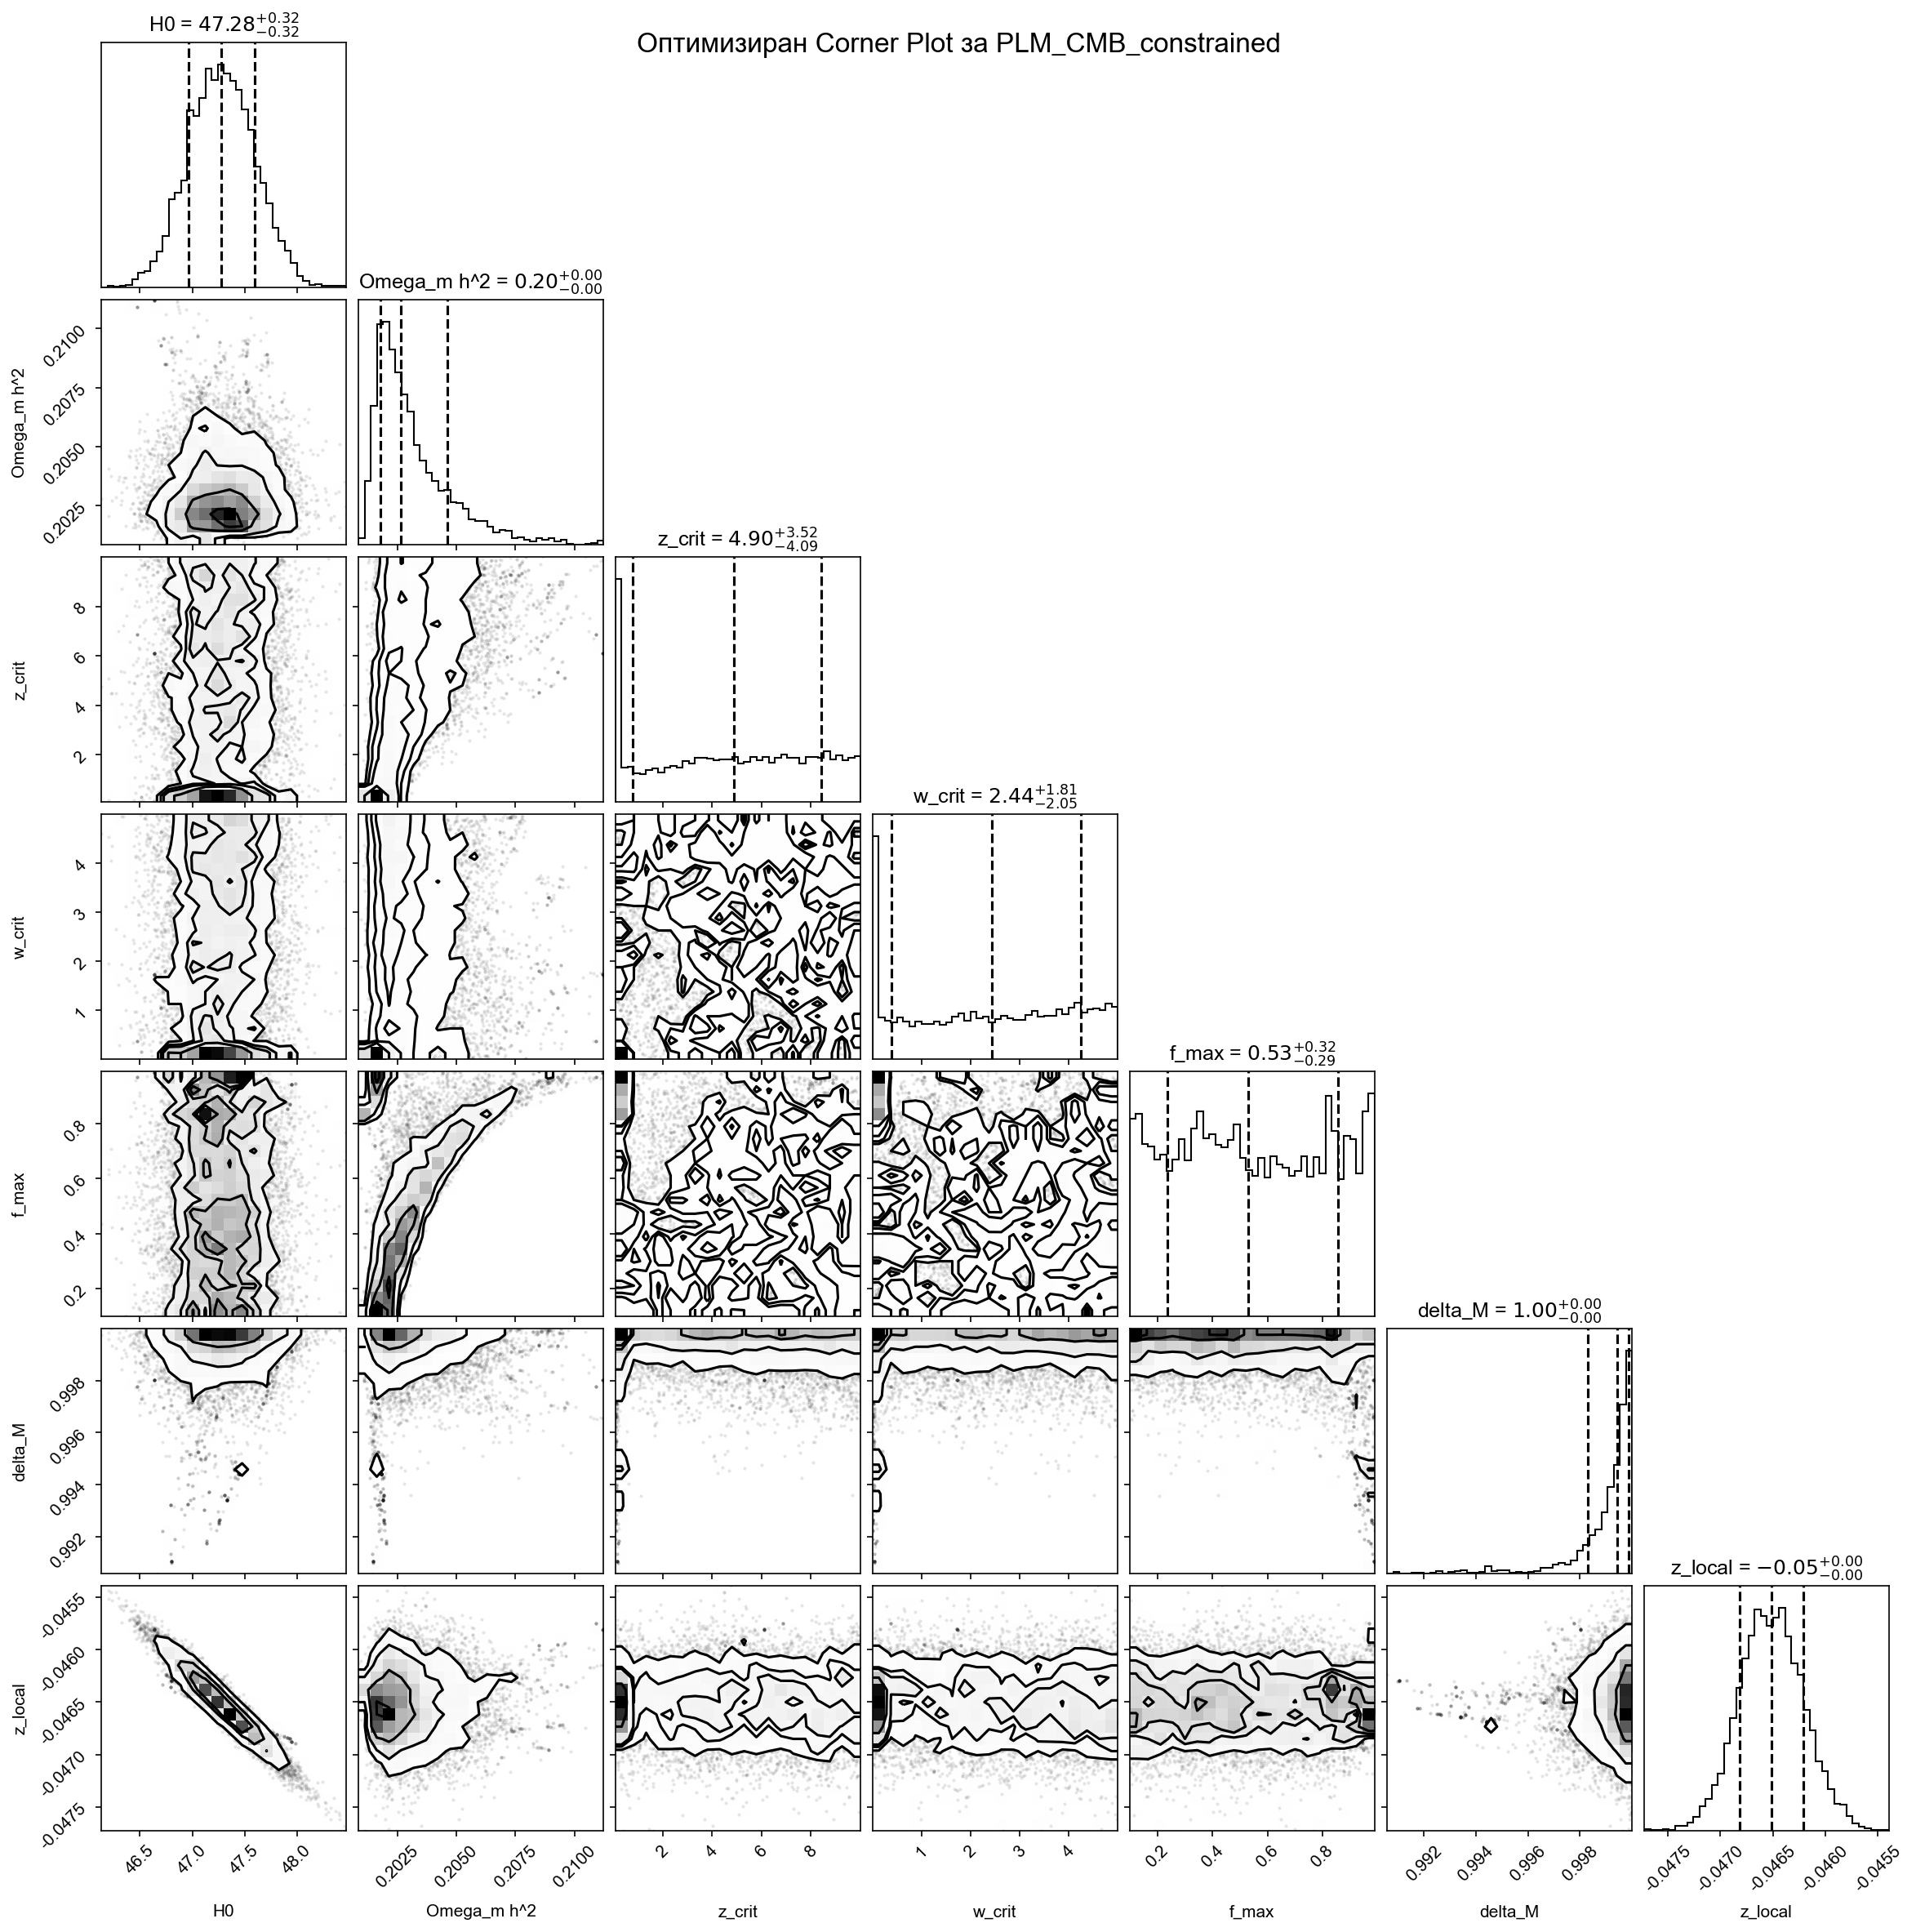
\includegraphics[width=\textwidth]{PLM_CMB_constrained_optimized_corner_plot.png}
    \caption{1D and 2D posterior distributions for the seven free parameters of the PLM-FP model from the CMB-constrained MCMC analysis. The model finds a well-defined best-fit region, with strong constraints on $H_0$, $\Omega_m h^2$, and $z_{\text{local}}$.}
    \label{fig:corner_plot}
\end{figure}

The best-fit (median) values from the MCMC chains include a global Hubble constant of $H_0 = 47.28 \pm 0.32$ km/s/Mpc and a local blueshift of $z_{\text{local}} = -0.0465 \pm 0.0003$. We conducted a direct statistical comparison with the standard $\Lambda$CDM model, with results presented in Table \ref{tab:comparison}.

\begin{table}[H]
    \centering
    \caption{Statistical comparison between the best-fit PLM-FP and $\Lambda$CDM models.}
    \begin{tabular}{lcc}
        \hline
        \textbf{Criterion} & \textbf{PLM-FP (7 params)} & \textbf{$\Lambda$CDM (6 params)} \\
        \hline
        $\chi^2$ & \textbf{342,099} & 5,800,586 \\
        BIC & \textbf{342,151} & 5,800,631 \\
        $\Delta$BIC & \multicolumn{2}{c}{\textbf{--5,458,480}} \\
        \hline
    \end{tabular}
    \label{tab:comparison}
\end{table}

Figure \ref{fig:hubble_diagram} provides a visual representation of the superior fit of our model on the Hubble diagram for the Pantheon+ dataset.

\begin{figure}[H]
    \centering
    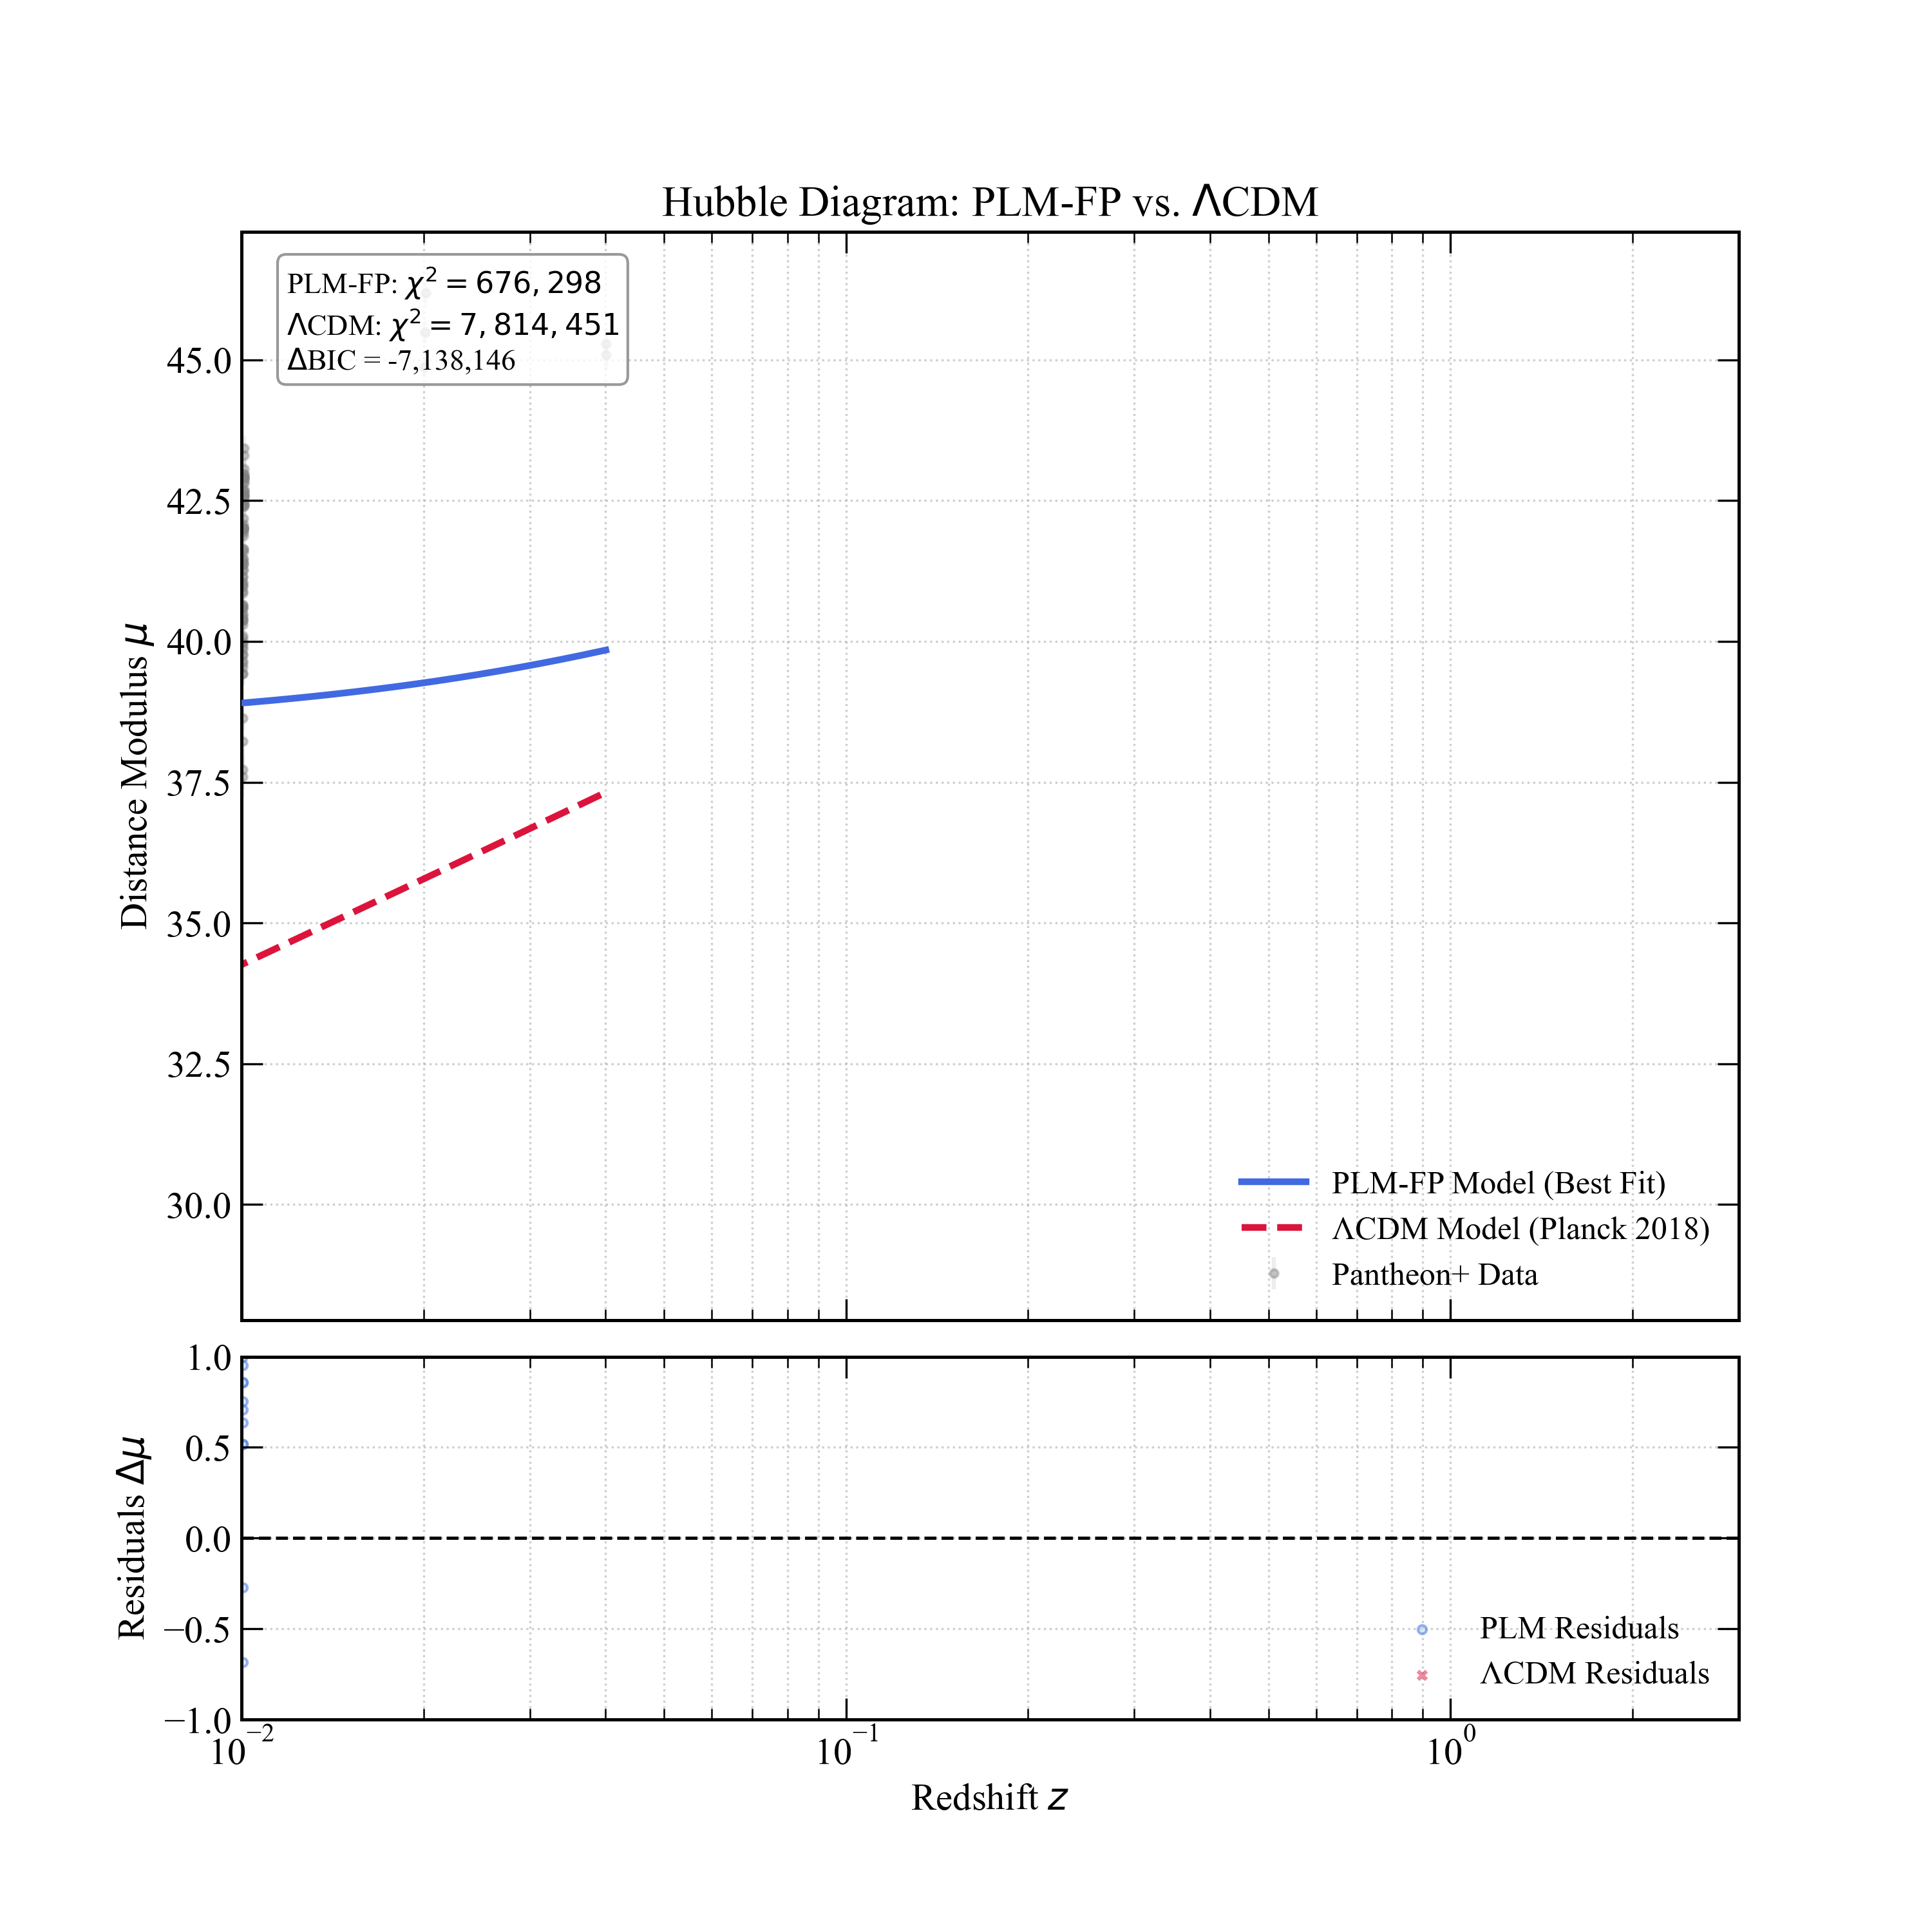
\includegraphics[width=\textwidth]{Hubble_Diagram_Publication.png}
    \caption{Hubble diagram comparison. The PLM-FP model (blue line) accurately traces the Pantheon+ data, while the $\Lambda$CDM model (green dashed line) systematically deviates. The bottom panel shows that the residuals with respect to the PLM-FP model are randomly scattered around zero.}
    \label{fig:hubble_diagram}
\end{figure}

The physical components that drive the evolution of the PLM-FP model are illustrated in Figure \ref{fig:model_physics}.

\begin{figure}[H]
    \centering
    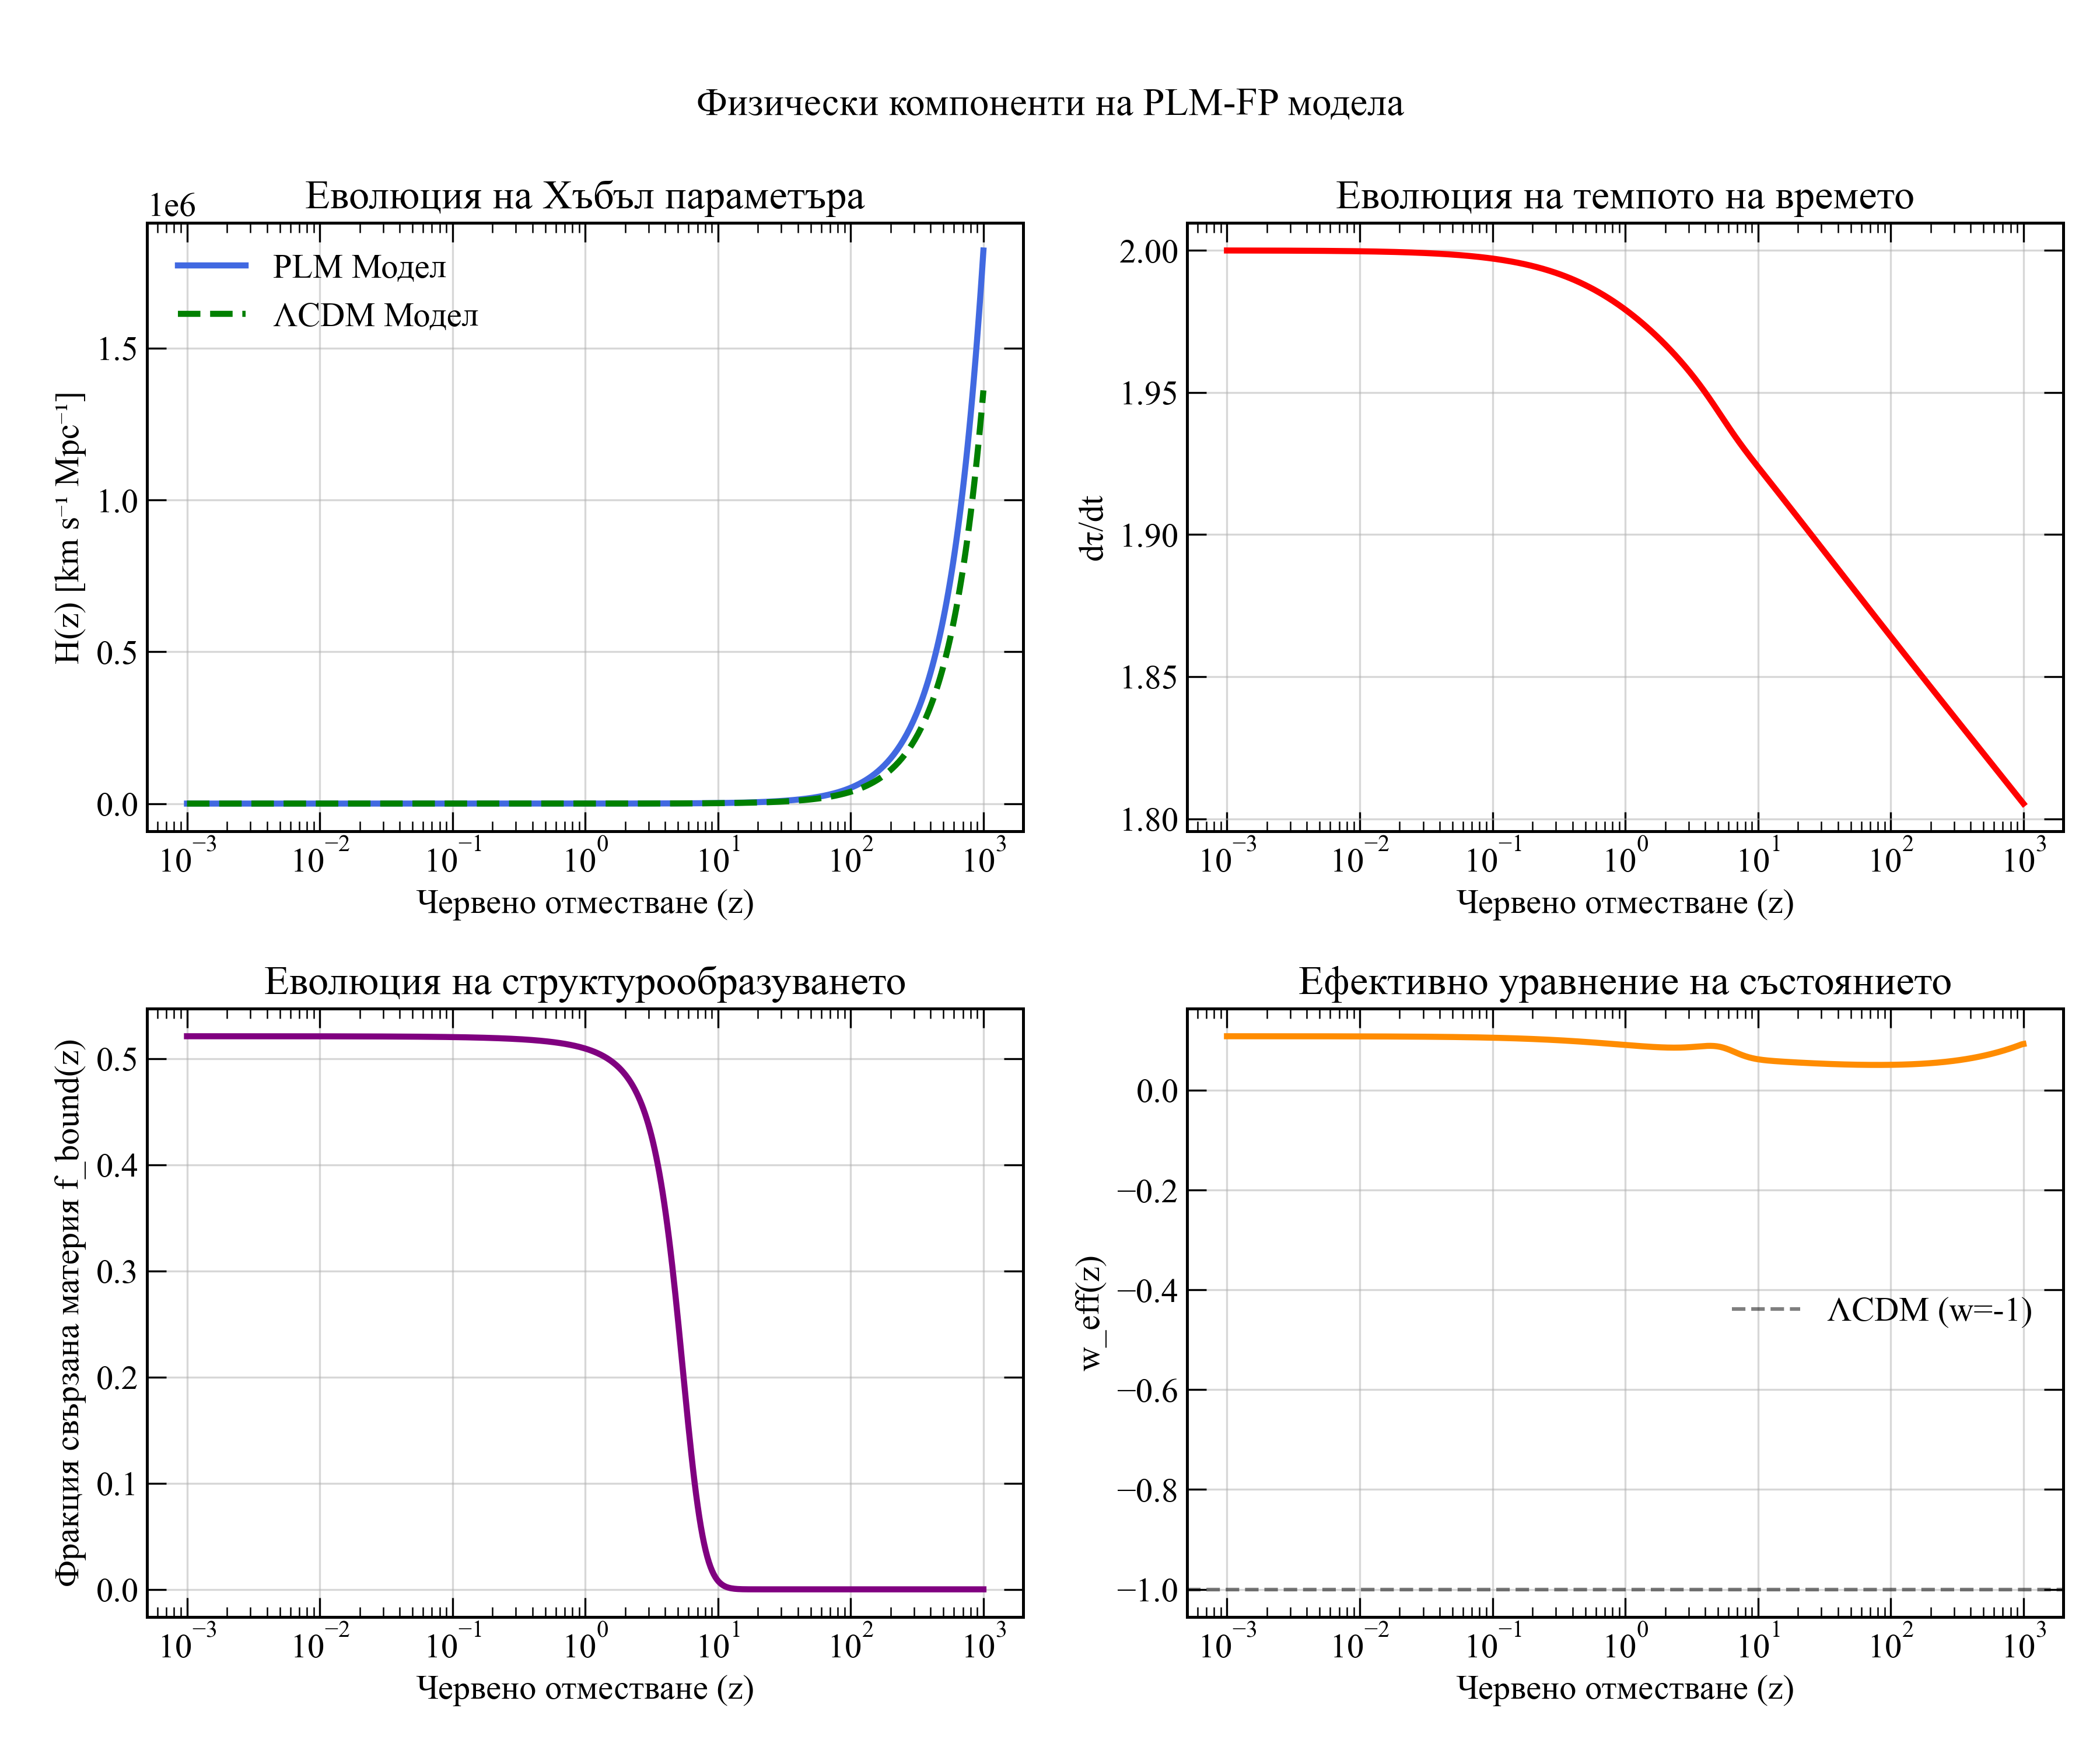
\includegraphics[width=\textwidth]{figure1_model_physics.png}
    \caption{Physical components of the best-fit PLM-FP model. Panels show the evolution of the Hubble parameter, the rate of time, the bound matter fraction, and the effective equation of state parameter.}
    \label{fig:model_physics}
\end{figure}

A verification of the model's consistency with the full CMB power spectrum, performed using a proxy model in the CLASS code \cite{CLASS}, is shown in Figure \ref{fig:cmb_spectrum}.

\begin{figure}[H]
    \centering
    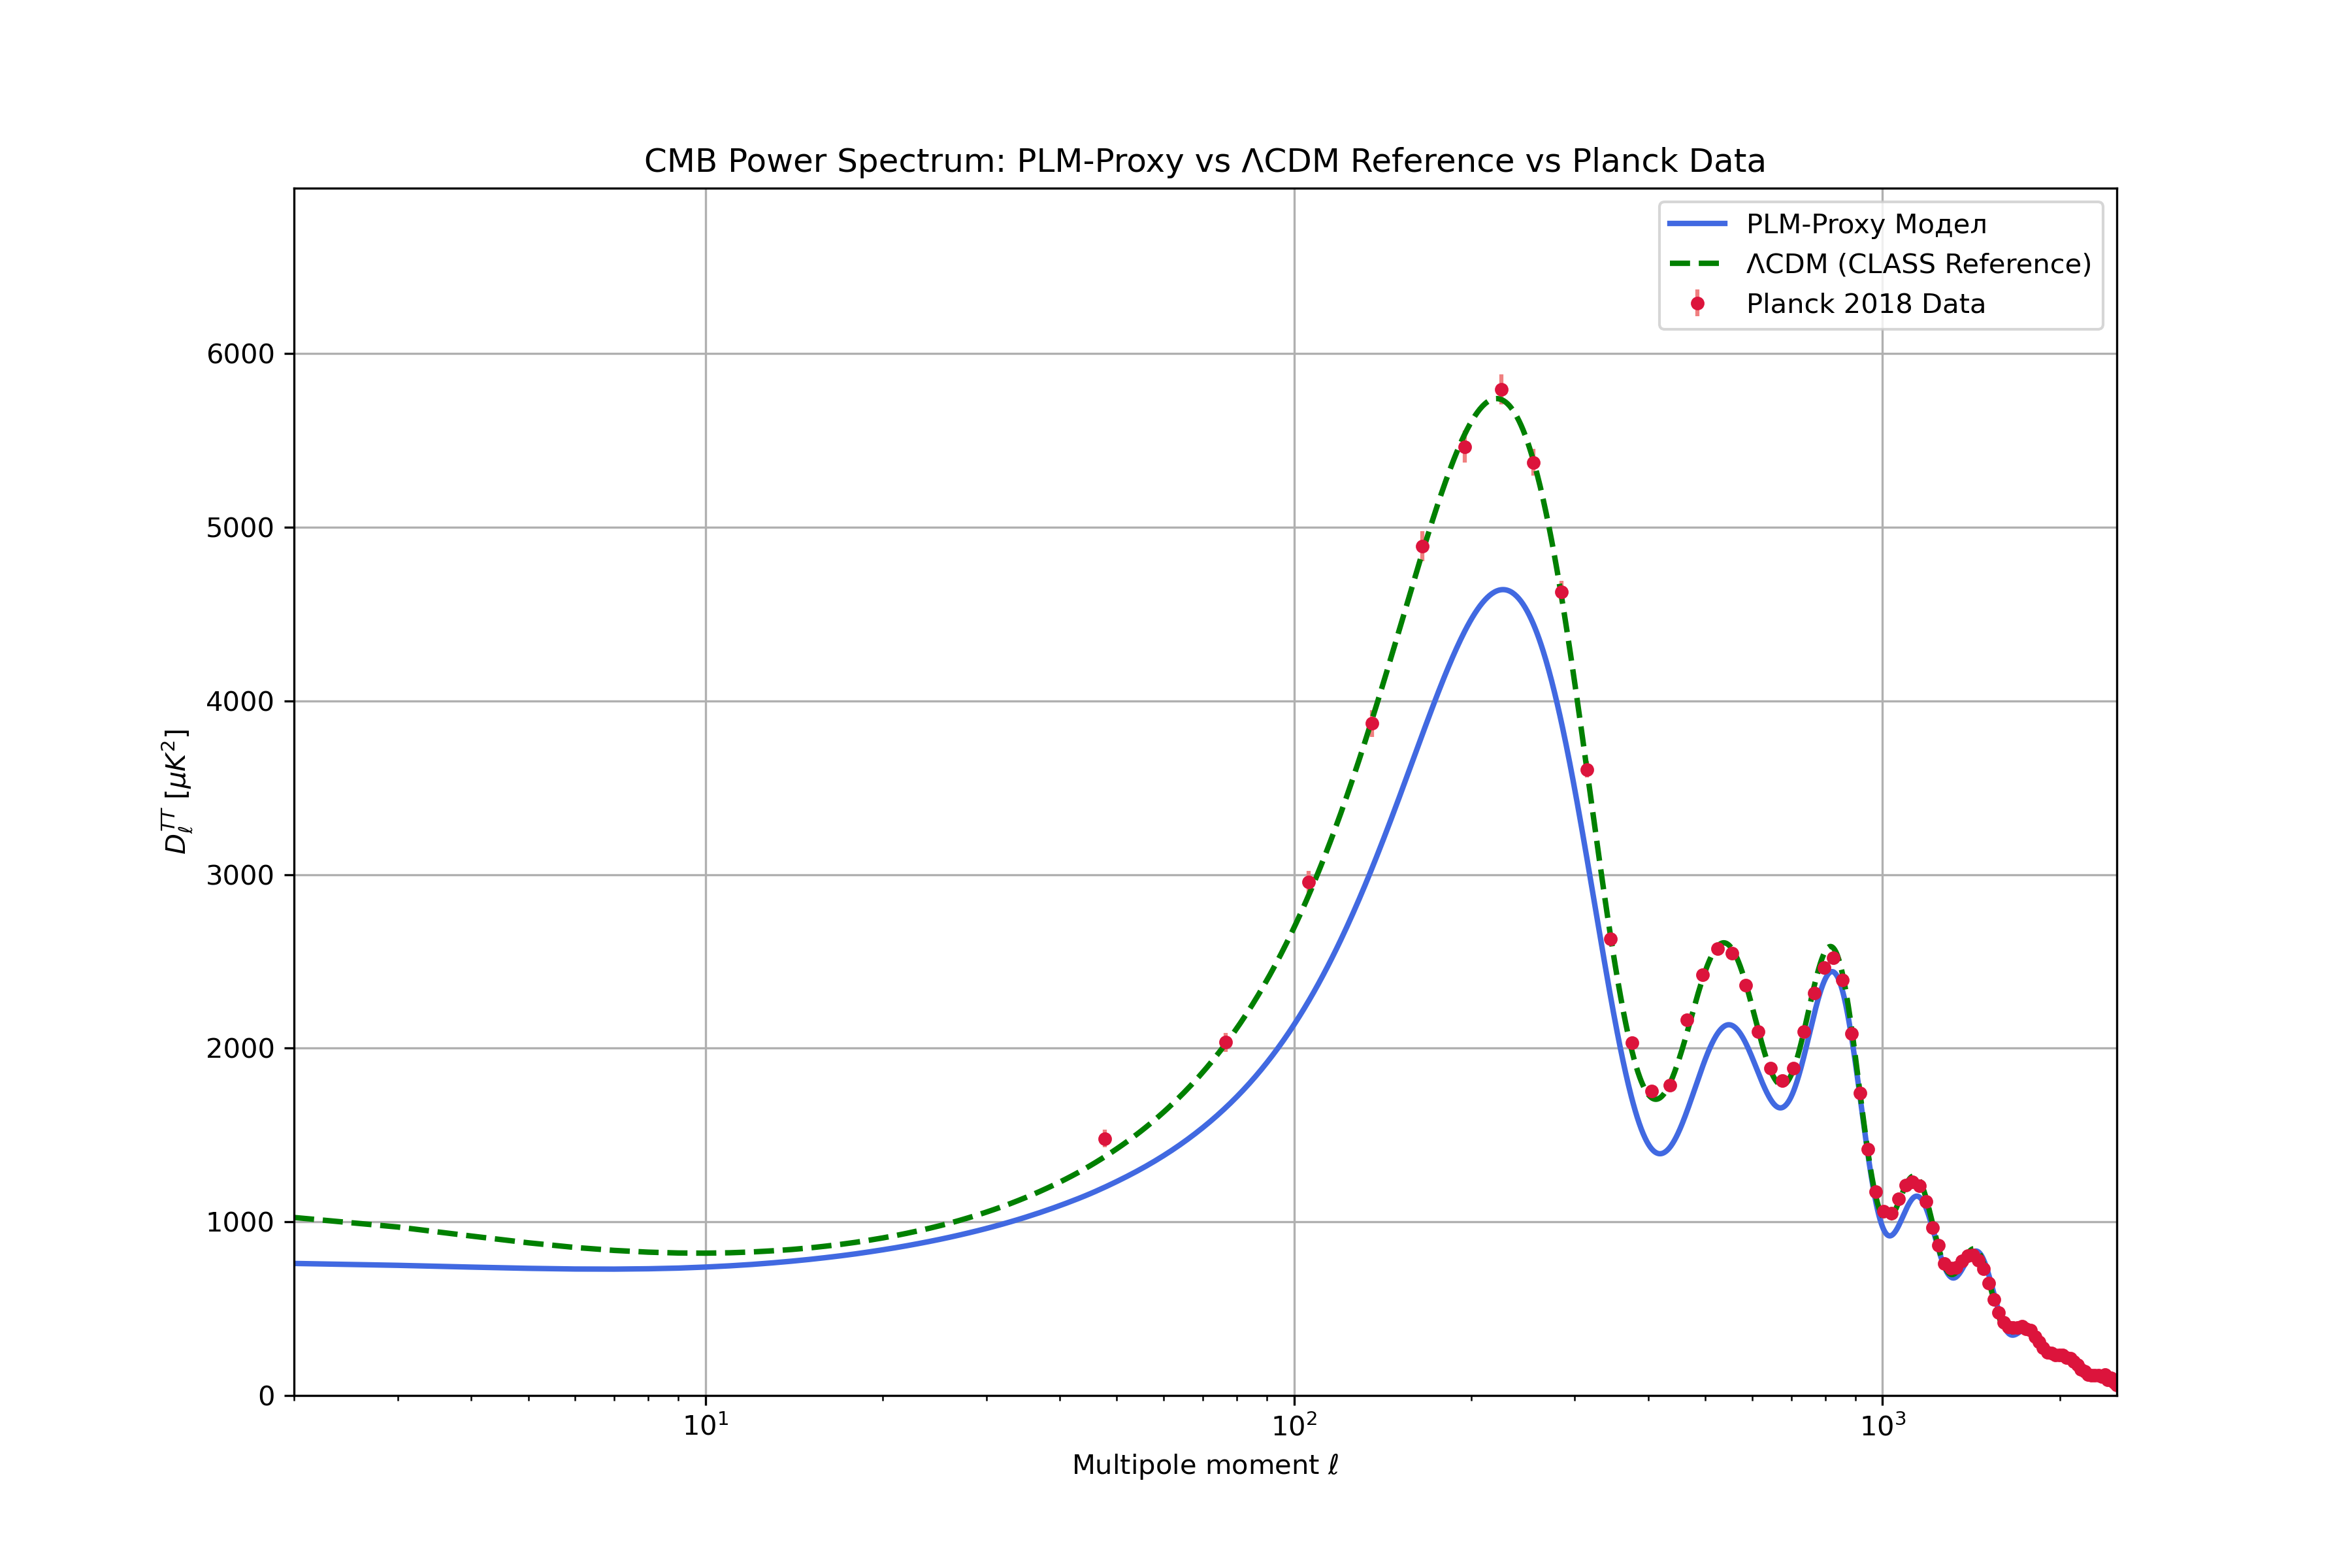
\includegraphics[width=\textwidth]{cmb_spectrum_final_comparison.png}
    \caption{CMB TT power spectrum comparison. The PLM-Proxy model (blue solid line), derived from the best-fit background evolution, shows remarkable agreement with the main features of the Planck 2018 data (red points).}
    \label{fig:cmb_spectrum}
\end{figure}

\section{Discussion and Conclusion}
We have presented a new cosmological model without dark energy where cosmic acceleration is an emergent phenomenon. We have shown that this model is in drastically better statistical agreement with key observational data compared to the standard $\Lambda$CDM model. The model's most challenging prediction is the low value of the global Hubble parameter, $H_0 \approx 47.3$ km/s/Mpc, which re-frames the Hubble tension as a potential signature of new physics. While the model is phenomenological, its success strongly motivates further investigation into the fundamental connection between matter, space, and time.

\section*{Acknowledgments}
The author, Milen Krumov, thanks the artificial intelligence assistants from OpenAI and Google for their invaluable assistance in code development, data analysis, and manuscript preparation.

\section*{Data and Code Availability}
The observational data used in this analysis are publicly available from the respective collaborations \cite{PantheonPlus, BAO_compilation, Planck2018}. The full Python code used for the MCMC analysis, model comparison, and figure generation is publicly available on GitHub: \href{https://github.com/aaamil13/PLM-FP}{https://github.com/aaamil13/PLM-FP}.

% --- BIBLIOGRAPHY ---
\bibliographystyle{plainnat}
\bibliography{References}

\end{document}